\section{Theory}

	\subsection{Fabry-Perot Interferometer}
		The Fabry-Perot Interferometer utilizes the phenomena of interference of multiple beams of light coming from a source that interferes with a screen. The wavelength of the light can be determined from the circular interference fringes of equal inclination formed on the screen. Other than that the interferometer is also used to find small differences in different wavelengths of light coming from a source, etc. The light coming from the source is bro- ken down into multiple beams as it continuously reflects between the high reflecting surface of two etalon plates while transmitting a portion of it through every reflection. The fringes are formed due to interference between these two beams when they are focused on a screen using a convex lens.

		\begin{figure}[H]
			\centering
			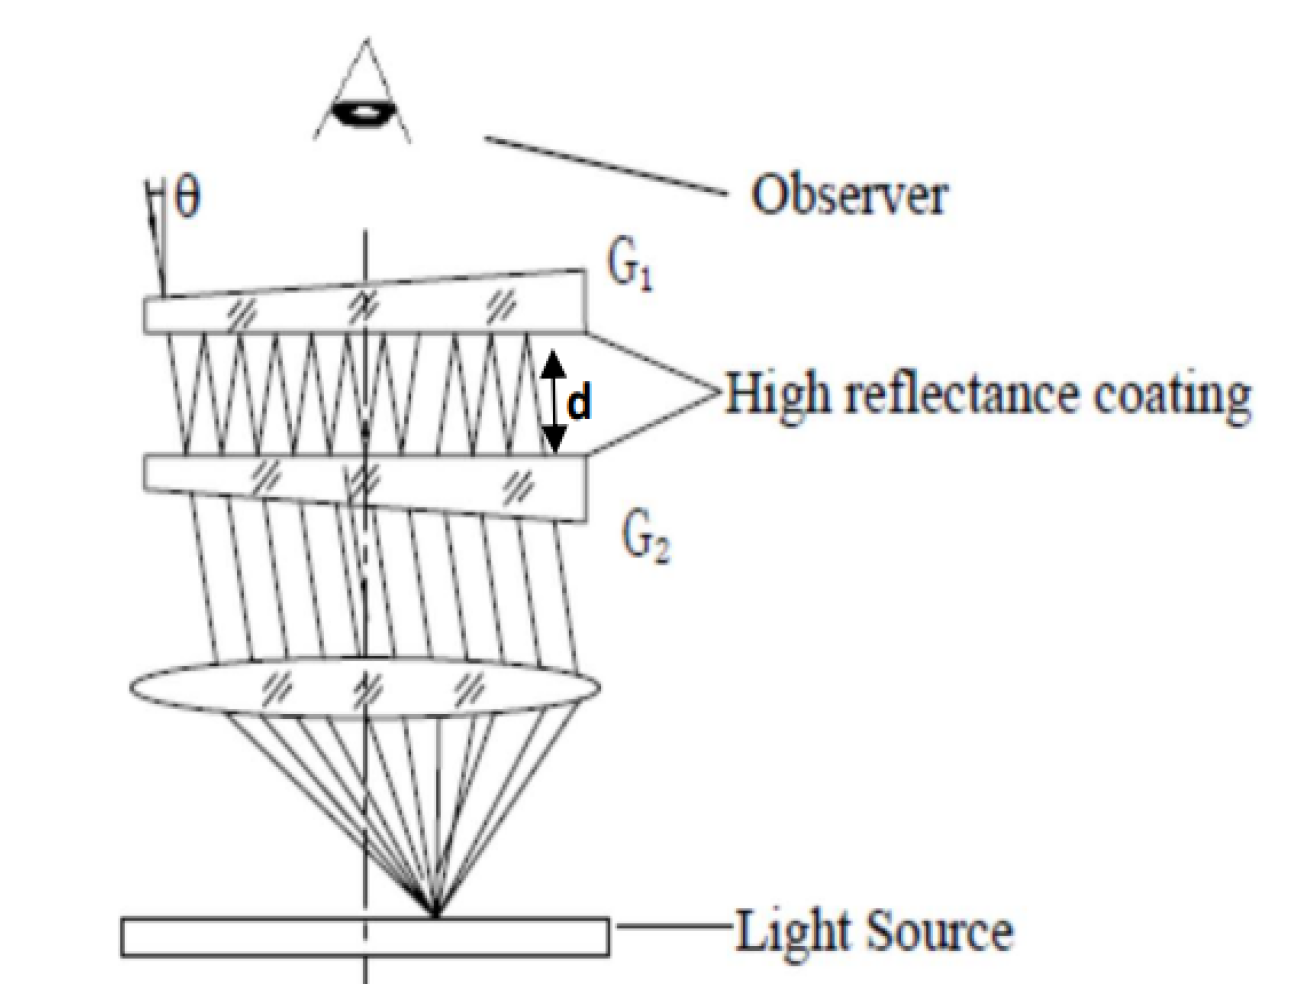
\includegraphics[width=0.45\textwidth]{images/febry_perrot.png}
			\caption{Schematics of a Fabry-Perot Interferometer}
			\label{fig:1}
		\end{figure}

		The components of the beam emerge parallel from $G_2$ at an angle of inclination theta with respect to the plate's surface, which is equal to the angle of inclination of the original beam striking the mirror $G_1$, as shown in the \hyperref[fig:1]{Figure 1}. The convex lens's focal plane, where the parallel rays are now focused, is on the screen. Because the angle of the rays determines where the interference occurs. The corresponding interference regions from a circular are seen for the rays with the same inclination on the plates in all directions. These fringes are known as fringes of equal inclination because each circular figure corresponds to a specific inclination. The interference pattern exists due to the path difference ($\Delta$) any two interfering rays of wavelength ($\lambda$), given by the equations:

		\begin{itemize}
			\item Constructive Interference: $\Delta = n\lambda$, $[n\in\mathbb{Z}]$
			\item Destructive Interference: $\Delta = \frac{(n+1)\lambda}{2}$, $[n\in\mathbb{Z}]$
		\end{itemize}

		Each interference maximum is caused by a corresponding ray path difference that depends on inclination and is therefore specific to each fringe. T the following path difference between two interfering beams (see \hyperref[fig:2]{Figure 2}) can be calculated, one from direct transmission through $G_1$ and the other from two successive reflections in the air gap:

		\begin{figure}[H]
			\centering
			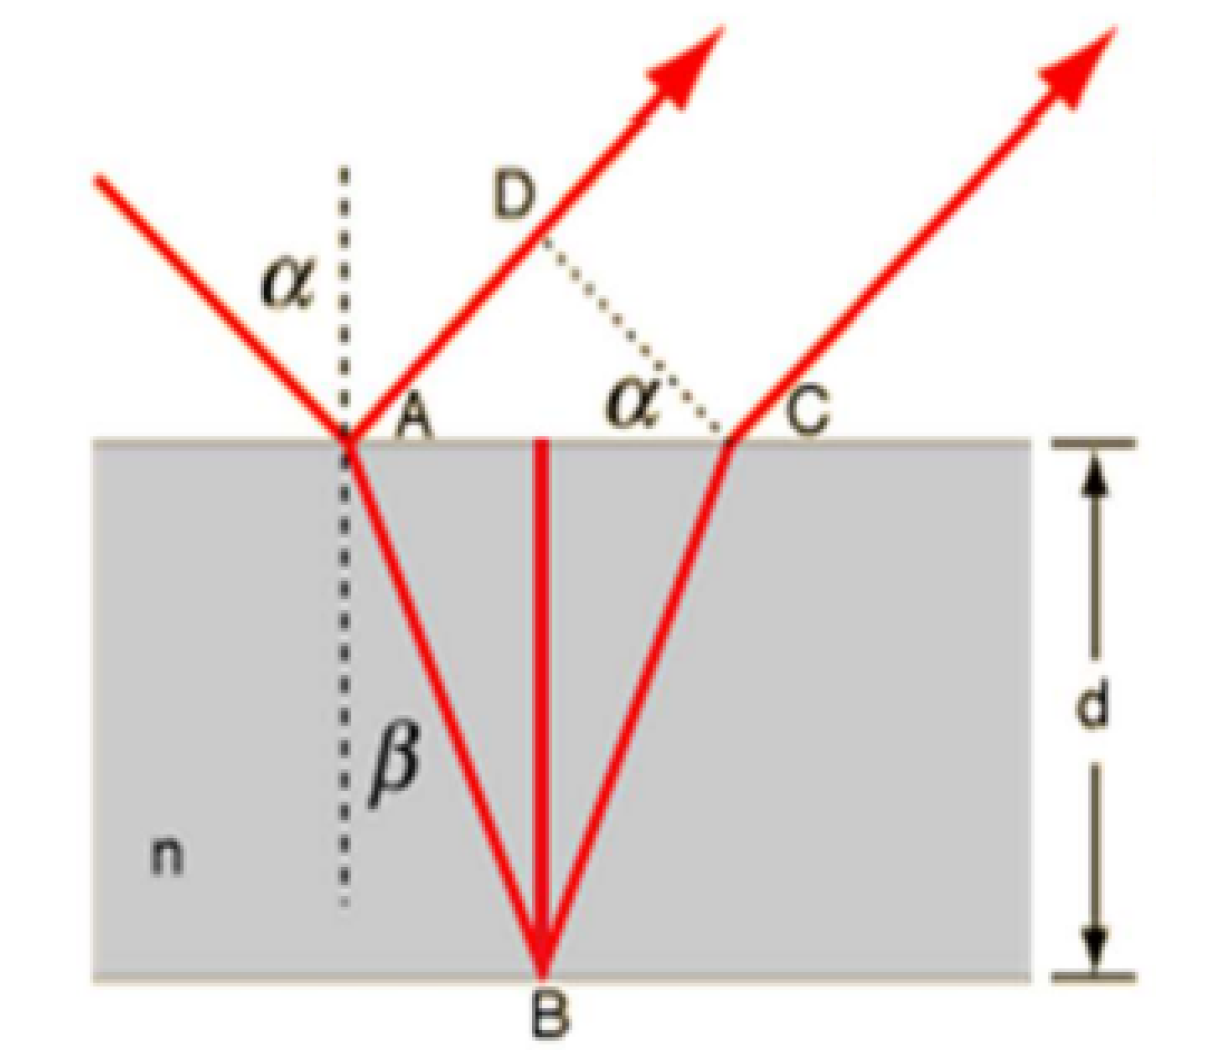
\includegraphics[width=0.45\textwidth]{images/path_difference.png}
			\caption{Calculation of Path Difference}
			\label{fig:2}
		\end{figure}

		In the \hyperref[fig:2]{Figure 2} the the reflected wavefront from C interferes with the wavefront from C. Hence the path difference between the two interfering beams is given by $\Delta = n(AB + BC) - AD$ [$n(\approx 1$ for air) is the refractive index of the medium]. d is the distance between the two etalons and $\beta$ is the angle of incidence of the beam on the second etalon. On putting the values of the variables in the equation AB, BC and DC in terms of $\beta$, we get:

			$$\Delta = 2nd\cos\beta$$

	\subsection{Determination of Wavelength $(\lambda)$:}

		For some light rays with the same inclination, the path difference changes as the distance between the plates changes. A maxima will be seen for a lower inclination for an increased $d$, while maxima for a decreasing $d$ will vanish. The change in path difference will equal to an integer multiple of the wavelength of light for each recurrence of maxima at the same inclination. As a result, for small values of beta, the wavelength is given by (from the constructive interference formula):

		\begin{equation}
			\lambda = \frac{2(d_2-d_1)}{m_2-m_1} = 2\times slope
			\label{eq:1}
		\end{equation}

		Where $d_2$ and $d_1$ are the final and initial position of the
		fine micrometer respectively used for adjusting $d$; and
		$(m_2 - m_1)$ is the number of fringes appearing or disappearing
		at the centre, that is inclination of $0^\circ$.

	\subsection{Determination of distance between the plates $(d)$:}

		We know $\Delta = 2d\cos\theta_m$ for $\theta_m$ being the inclination of the m-th fringe. Therefore using small angle approximation:

			$$\theta_m = \frac{r_m}{D}$$

		here, $r_m$ is radius of the m-th fringe and $D$ is the distance between the etalon and the screen. For the m-th fringe, the path difference $\Delta = m\lambda$ implies:
		
		\begin{equation}
			d= \frac{m\lambda}{2\cos\theta_m}
			\label{eq:2}
		\end{equation}

		\begin{figure}[H]
			\centering
			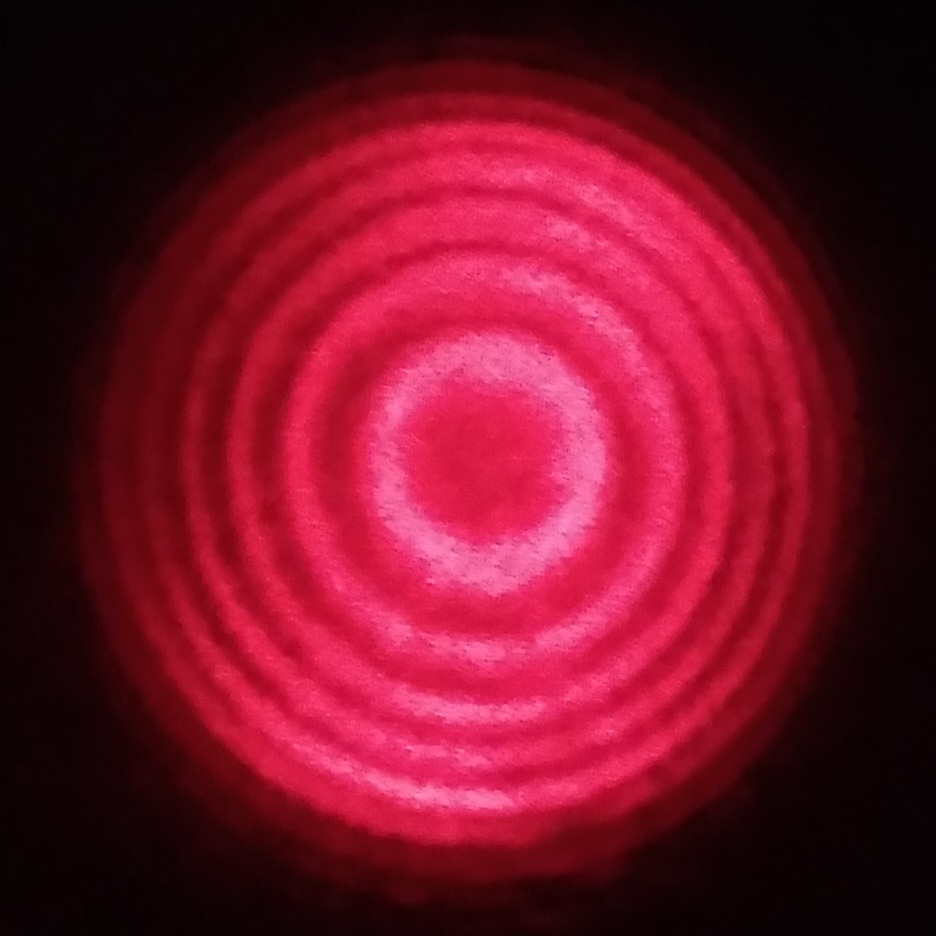
\includegraphics[width=0.45\textwidth]{images/1.jpg}
			\caption{Circular fringes}
			\label{fig:3}
		\end{figure}